\documentclass[10pt,twocolumn]{article}

\usepackage[margin=30pt]{geometry}
\usepackage{amsmath}
\usepackage{physics}
\usepackage{amssymb}
\usepackage{amsfonts}
\usepackage{hyperref}
\usepackage{thmbox}
\usepackage{geometry}
\usepackage{graphicx}
\usepackage[]{subcaption}

\newcommand{\R}{\mathbb{R}}
\newcommand{\C}{\mathbb{C}}

\author{Haiyang Wang, Nils Jan Fredrik Fryklund, Samuel Potter, Leslie Greengard}
\date{\today}
\title{A Fast Solver for Stokes Flow in 2D: [this is a bad title]}

\begin{document}

\maketitle

\begin{abstract}
  In this paper, we exploit the \textit{return to Poiseuille} phenomenon: 
  a flow would gradually developed into the Poiseuille flow along a straight channel. 
  This allows us to quickly build a solver for the interior plane Stokes flow
  with a domain that is union of \textit{standard pieces}. 
  Each standard piece's is a pipe with inlets/outlets 
  being long enough straight channels, so that when two standard pieces are connecting, 
  the velocity profile at where they connect would be close to Poiseuille flow velocity profile up to machine precision. 
  \footnote{The length of straight channel is greater than 7 times of the width, as indicated by Figure \ref{fig:r2pnumerical} }
  Therefore, we can solve the Stokes equation for each standard pieces with Poiseuille boundary condition at inlets/outlets, and then easily interface the local solutions of each standard pieces to build a solution for the global domain.  
  
  Once we pre-built the solvers for each standard piece, 
  it is numerically stable to connect these standard pieces to form 
  a large and complex pipe network. 
  The connection algorithm is based on 
  the physics constraints of  zero-net-flux and continuity of pressure. 
  Connecting the local solvers would have time complexity of $O(n^2)$, 
  where $n$ is the number of standard pieces. 
  This is much faster than solving the global problem directly, which demands at least $O(N)$ time complexity. 
  More specifically, for the numerical example in Figure [to be included], connecting the local solutions took only 0.3 seconds, and directly solving for the global domain would take 24 minutes. 
  
\end{abstract}

\section{Introduction}


For plane Stokes flow, the biharmonic equation formulation are well known 
and developed within theory of complex variable from the last century \cite{ladyzhenskayaMathematicalTheoryViscous1964}. 
Various numerical schemes, such as boundary integral equation (BIE) and rational function approximation, 
have been developed accordingly \cite{greengardIntegralEquationMethods1996,trefethenApproximationTheoryApproximation2019}. 

The \textit{return to Poiseuille} phenomenon, or \textit{Saint-Venant's principle} in the theory of plane elasticity, 
are well-established from the last century 
\cite{coRecentDevelopmentsConcerning1983,gregoryTractionBoundaryValue1980,horganDECAYESTIMATESBIHARMONIC1989}. 
To be more specific, in a straight channel with laminar and incompressible incoming flow, the differences of Stokes flow and Poiseuille flow would decay exponentially fast toward the outlet. 
Therefore it is a good numerical hypothesis to assume that the flow is Poiseuille in middle of a lone straight channel.

% TODO : maybe move this sentence to the numerical experiment part. 
% The BIM is coupled with the biharmonic Fast Multiple Method (FMM) 
% to reduce space and time complexity for the matrix-vector product \cite{FlatironinstituteFmm2d2022}.

In this paper, we use the boundary integral method (BIM) from 
\cite{greengardIntegralEquationMethods1996} to build solvers for multiple standard pieces 
with Poiseuille boundary condition in at inlets/outlets. 
Directly evaluating the BIM's solution near the boundary could be numerically unstable as the integral is nearly-singular.
Thus, we have adopted the methods from 
\cite{wuSolutionStokesFlow2020,helsingEvaluationLayerPotentials2008} 
to for stable evaluation of layer potentials near the boundary. 
Finally, connection of standard pieces is by simply solving a system of linear equations, 
from the physics law of zero-net-flux and single-valued-ness of pressure. 
This linear equation depends merely on the flux and pressure at the
point of connection of standard pipes, therefore can be solved instantly. 

This paper is organized as follows. In Section \ref{mathprelim}, we define the Stokes boundary value problem, 
the corresponding biharmonic boundary value problem, and then the integral equation of it. 
We also mention the analytic evidence for the \textit{return to Poiseuille} hypothesis. 
In Section \ref{sec:numericalmethod}, we presents the Nystr\"om discretization
of the integral equation. 
The numerical experiments of connecting standard pieces and numerical evidence for \textit{return to Poiseuille}
hypothesis are contained in Section \ref{sec:numericalresults}, 
followed by conclusions in Section \ref{sec:conclusions}.

\section{Mathematical Preliminaries\label{mathprelim}}

In this section, we first state the Stokes equation, translate it into the biharmonic equation,
and then derive the Boundary Integral equation. This whole derivation is nothing new from \cite{greengardIntegralEquationMethods1996}. 
Then, we will present an analytic estimate for the exponential rate of 
\textit{return to Poiseuille} \cite{gregoryTractionBoundaryValue1980}. 

\subsection{Stokes Boundary Value Problem}

The plane linear Stokes equations are
\begin{align}
  \nu \Delta u = \frac 1 \rho \pdv{p}{x},\quad &\nu \Delta v = \frac 1\rho \pdv{p}{y} 
  \label{stokes} \\
  \pdv{u}{x} + \pdv{v}{y} &= 0
  \label{continuity}
\end{align}
where $u,v$ are components of velocity, 
$\rho$ is the density, 
$\nu$ is the viscosity, 
and $p$ is the pressure. 
Another important physics quantity, vorticity, is defined as $\zeta  = u_y - v_x$. 


We are interested in interior boundary value problem on a finite $(M+1)$-ply connected domain $D\subset \mathbb R^2$,
with boundary $\partial D =  \Gamma = \Gamma_0 \cup \Gamma_1 \cup \cdots \cup \Gamma_M$, 
where $\Gamma_0$ is the exterior boundary, and $\Gamma_1,\cdots, \Gamma_M$ are the interior boundaries. We restrict our attention to 
problems where the velocity is defined by given function $h_1,h_2$ on the boundary:
\begin{align}
  u = h_2(t),\quad v = - h_1(t), \quad t\in \Gamma
  \label{bdr-velocity}
\end{align}

\subsection{The Biharmonic Potential}

In this section, 
we briefly review the biharmonic potential of plane Stokes flow, 
the Goursat's representation of biharmonic function, 
the Sherman-Lauricella representation, 
and the BIE to be solved numerically
\cite{ladyzhenskayaMathematicalTheoryViscous1964,greengardIntegralEquationMethods1996}. 

\paragraph*{Biharmonic Stream Function.} $(\ref{continuity})$ implies the existence of the stream function $W(x,y)$ such that:
\begin{align}
  \pdv{W}{x} = -v,\quad \pdv{W}{y} = u \label{stream-1}
\end{align}

Following (\ref{stokes},\ref{continuity}), it is easy to see that the stream function satisfies the biharmonic equation (\ref{biharmonic}),
and the boundary velocity conditions ($\ref{bdr-velocity}$) can be understood as the boundary conditions for the biharmonic equation (\ref{bih-bv}):
\begin{align}
  &\Delta^2 W(x,y) = \Delta \zeta = 0, &(x,y)\in D \label{biharmonic}\\
  &\pdv{W}{x}(t) = h_1(t),\quad \pdv{W}{y}(t) = h_2(t), \quad &t\in \Gamma\label{bih-bv}
\end{align}
where $h_1,h_2$ are from equation (\ref{bdr-velocity}).

\paragraph*{Goursat's Formula.} It has been long established that any plane biharmonic function $W(x,y)$ can be expressed by Goursat's formula 
\begin{align}
  W(x,y) = \Re (\bar z \phi(z) + \chi (z)) \label{Goursat}
\end{align}
where $\phi, \chi$ are analytic functions of complex variable $z = x+yi$. 
In the following, we will be identifying $(x,y) \in \mathbb{R}^2$ with $x + yi\in \mathbb{C}$. 


The Muskhelishvili's formula connects velocity of Stokes flow with the Goursat's formula \cite{muskhelishviliBasicProblemsMathematical1977}: 
\begin{align}
    u(x,y) + iv(x,y) 
    &= \phi(z) + z \overline{\phi'(z)} + \overline{\psi(z)}
    \label{muskhelishvili}
\end{align} where $\psi = \chi'$. This transforms the biharmonic boundary condition \eqref{bih-bv} into 
\begin{align}
  \phi(t) + t\overline{\phi'(t)} + \overline{\psi(t)} 
  = h(t), \quad
  t \in \Gamma
\end{align} where $h(t) =  h_1(t) + ih_2(t)$,  and $t$ is understood as a complex variable. 

For Stokes flow, there is another formula connecting pressure and vorticity with 
the Goursat's functions
\begin{align}
  \zeta + \frac{i}{\nu}p = 4\phi'(z) \label{pressure-and-vorticity}
\end{align}


\paragraph*{Sherman-Lauricella Representation.} The boundary integral equation is an ansatz 
based on of an extension of Sherman-Lauricella representation 
proposed in \cite{greengardIntegralEquationMethods1996}. 
It is formulated as follows:
\begin{align}
  \phi(z) &=
    \frac {1}{2\pi i} \int_\Gamma \frac{\omega(\xi)}{\xi - z} d\xi  
    + \sum_{k=1}^M C_k \log (z-z_k)
    \\
  \psi(z) &=
    \frac {1}{2\pi i} \int_\Gamma \frac{\overline{\omega(\xi)}d\xi +  \omega(\xi)\overline{d\xi}}{\xi - z}  
    - \frac {1}{2\pi i} \int_\Gamma \frac{\overline{\xi} \omega(\xi)}{(\xi - z)^2} d\xi  
    \\
    & \quad + \sum _{k=1}^M 
    \left( \frac{b_k}{z-z_k} + \overline C_k \log (z-z_k) -  C_k \frac{\overline z_k}{z-z_k} \right) \nonumber 
\end{align}
where $\omega$ is an unknown complex density on $\Gamma$ to be solved for, 
$z_k$ are arbitrarily prescribed point inside the component curves $\Gamma_k$, 
and $C_k, b_k$ are constants defined by 
\begin{align}
  C_k = \int_{\Gamma_k} \omega(\xi) |d\xi|, \quad b_k = 2 \Im\int_{\Gamma_k} \overline{\omega(\xi)} {d\xi}
\end{align}

\paragraph*{Boundary Integral Equation.} 
Letting a point $z$ in the interior of $D$ approach to a point on the boundary $t\in \Gamma$, 
the classical formulae for the limiting values of Cauchy-type integral 
gives us the an integral equation for $\omega$ \cite{muschelisviliSingularIntegralEquations1972,greengardIntegralEquationMethods1996} :
\begin{align}
  \omega(t) 
  &+ \frac 1{\pi } \int_{\Gamma} \omega(\xi) d\ln \frac{\xi - t}{\overline{\xi - t}} - \frac 1{2\pi i} \int_\Gamma \overline{\omega(\xi)} d \frac{\xi - t}{\overline{\xi - t}} \label{bie} \\
  &+ \sum_{k=1}^M \left( \frac{\bar b_k}{\overline{t- z_k}} +  2C_k \log |t-z_k| + \bar C_k \frac{t-z_k}{\overline{ t - z_k}} \right) \nonumber\\
  &+ \frac{\overline b_0}{\bar t - \bar z^*} \nonumber \\
  &= h(t) \nonumber
\end{align}
the extra term $\frac{\overline b_0}{\bar t - \bar z^*}$ vanishes when the zero-net-flux condition $\Re \int_\Gamma \bar h(t) dt = 0$ is satisfied. 
The invertibility of this integral equation is similar 
to the standard proof of invertibility for elasticity problems \cite{muskhelishviliBasicProblemsMathematical1977}, hence omitted.

\subsection{Return to Poiseuille\label{sec:ret2poi}} 

In this section, we will first show the analytic estimate for the \textit{return to Poiseuille} phenomenon,
which is from the eigenfunction analysis on a semi-infinite strip from the theory of plane elasticity 
\cite{gregoryTractionBoundaryValue1980}. 
Then, we explain how to apply the \textit{return to Poiseuille} hypothesis. 

\paragraph*{Analytic Estimate for Return to Poiseuille. }

On the domain of a semi-infinite pipe $D_L = \{(x,y)\mid x \ge 0, |y| \le L\}$, with the boundaries 
\begin{align}
  \Gamma_L &= \Gamma_L^1 \cup \Gamma_L^2 \cup \Gamma_L^3 \\
  &=\{(0,y)||y| \le L \} \cup \{(x,L)|x\ge 0\} \cup \{(x,-L)\mid x\ge 0\}\nonumber
\end{align}
where $\Gamma_L^2,\Gamma_L^3$ are walls with the non-slippery boundary conditions, 
and $\Gamma_L^1$ is the inlet with boundary condition of an
incoming laminar incompressible flow. 
Return to Poiseuille means that regardless of the boundary conditions on $\Gamma_L^1$,
the flow's profile at $x = l$ will converge Poiseuille flow as $l$ approaches to infinity. 

Without lost of generality, assuming there is zero net flux across $\Gamma_L^1$,
return to Poiseuille is equivalent to return to zero flow. The equation for this BVP
is the following:
\begin{align}
  &\pdv{W(x,y)}{y}  = W(x,y) = 0,  &(x,y) &\in \Gamma_L^2 \cup \Gamma_L^3 \\
  &\pdv{W(0,y)}{x}  = f(y),\ \pdv{W(0,y)}{y} = g(y), &(0,y) &\in \Gamma_L^1  \label{eq:velocity-condition-at-inlet}
\end{align}
where $f,g$ satisfy $f(\pm L) = g(\pm L) = \int_{-L}^L g(y)dy = 0$. 

This biharmonic BVP is identical to the "self-equilibrated" traction BVP in the theory of elasticity studied in
\cite{gregoryTractionBoundaryValue1980,horganDECAYESTIMATESBIHARMONIC1989,coRecentDevelopmentsConcerning1983}. 
When $f''',g'''$ exist and are of bounded variation, 
this problem has a unique solution spanned by the Papkovich-Fadle eigenfunctions \cite{gregoryTractionBoundaryValue1980}.
The first eigenfunction is dominated by $e^{-xk/2L}$, where 
\begin{align*}
  k \simeq 4.2 
\end{align*}
is the smallest positive real parts of the roots 
of the transcendental equation $\sin^2\lambda - \lambda^2=0$. 
This gives the decay rate of return to Poiseuille hypothesis, 
which agrees with our numerical experiment in Figure \ref{fig:r2pnumerical}. 
% TODO

\paragraph*{Application of Return to Poiseuille.} Given the analytic bound, it is easy to see
that in a straight channel with length greater than 8 times of the channel width, we can expect the 
flow to be Poiseuille up to 14th digits accuracy. Therefore, it is appropriate to require the inlets/outlets of
the standard pieces to be such straight channels, and then assign the Poiseuille boundary conditions on them. 

The straight channels outlets would have two corners of right angle, making the geometry non-smooth. Such piecewise 
smooth geometry can be handled as in \cite{wuSolutionStokesFlow2020} with panel refinement near the corners. 
Here, we choose a different approach to avoid handling corners by adding superficial caps to the outlets. 
[this paragraph needs more elaboration and some figures perhaps]. 


\section{Description of Numerical Methods\label{sec:numericalmethod}}
In this section, we will first present Nystr\"om discretization of boundary integral equation (\ref{bie}), 
and then we briefly explain the discretization of the boundary, near boundary evaluation of layer potential, 
and the system of linear equations for pipe connections.  

\subsection{Boundary Integral equation}

The boundary curve $\Gamma_k$ is given by the parametrization $\Gamma_k = \{ t^k(a): a\in \left[A_k,A_{k+1}\right]\}$, 
and discretized into $N_k$ points $t^k_i = t^k(a^k_i)$. 
Associate to each point $t^k_j$ are the unknown complex density $\omega^k_j$, 
the derivative $d^k_j = t^{k\prime}(a^k_j)$, 
and the quadrature weight $w^k_j$. In total, we have $N= \sum_{k=0}^M N_k$ points. Nystr\"om discretization of (\ref{bie}) is
\begin{align}
  \omega_j^k 
  + \sum_{m=0}^{M}\sum_{n=1}^{N_k} K_1(t^k_j,t^m_n) \omega^k_j 
  + \sum_{m=0}^{M}\sum_{n=1}^{N_k} K_2(t^k_j,t^m_n) \overline{\omega^k_j} = h^k_j
  \label{nystrom}
\end{align} where $h^k_j = h(t^k_j)$ and the kernels $K_1, K_2$ are given by 
\begin{align}
  K_1(t^k_j, t^m_n) 
  &= \frac{1}{\pi} \Im (\frac{d^m_n}{t^m_n-t^k_j})w^m_n + K_1^s(t^k_j,t^m_n)\\
  K_2(t^k_j, t^m_n) 
  &= \frac{1}{\pi} \frac{\Im((t^m_n-t^k_j)\overline{d^m_n})}{(\overline{t^m_n - t^k_j})^2} w^m_n + K_2^s(t^k_j,t^m_n)
\end{align}
with $K_1^s, K_2^s$ being: 
\begin{align}
  K_1^s(t^k_j,t^m_n) &= \delta_m w^m_n \left(\frac{i\overline{d^m_n}}{\overline{t^k_j - z_m}}
  + 2 \log |t^k_j - z_m| \right)\\
  K_2^s(t^k_j,t^m_n) &= \delta_{m}w^m_n \left(- \frac{id^m_n}{\overline{t^k_j - z_m}} + \frac{t^k_j-z_m}{\overline{t^k_j - z_m}}\right) 
\end{align}
where $\delta_m = 1$ excepts for $\delta_0 = 0$. In the limiting case of $t^k_j = t^m_n$, the corresponding value can be seen as the limiting value:
\begin{align}
  K_1(t^k_j, t^k_j) &= \frac{w^k_j \kappa^k_j|d^k_j|}{2\pi} + K_1^s(t^k_j,t^k_j) \\
  K_2(t^k_j, t^k_j) &= -\frac{w^k_j\kappa^k_j(d^k_j)^2}{2\pi|d^k_j|} + K_2^s(t^k_j,t^k_j)
\end{align}where $\kappa^k_j$ is the signed quadrature at the point $t^k_j$. 

The left hand side (LHS) of (\ref{nystrom}) for any density $\omega$ is evaluated by a biharmonic fmm 
\cite{FlatironinstituteFmm2d2022}. 
And this Nystr\"om discretization is regarded as an matrix equation, 
by separating the real part and imaginary part, 
and then solved iteratively using 
generalized minimum residual method GMRES \cite{saadGMRESGeneralizedMinimal1986}. 

Evaluation of the layer potentials near boundary is done as in \cite{wuSolutionStokesFlow2020}. 

\subsection{Geometry of the Boundary}

The key to spectral convergence of GMRES is to have smooth boundary, 
or for piecewise smooth boundary, one can use special treatment as in \cite{wuSolutionStokesFlow2020}
to ensure the spectral convergence is preserved. Here for this paper, we focused on smooth geometry. 
We adopted the ideas from 
\cite{epsteinSmoothedCornersScattered2016,baggeHighlyAccurateSpecial2021} 
to smooth the corners of the boundary by convolution, and added superficial caps at the 
inlets and outlets. [insert a figure here]. The geometry is adaptively discretized into Gauss-Legendre panels, as described in
\cite{wuSolutionStokesFlow2020}. 


\section{Numerical Results and Discussion\label{sec:numericalresults}}
\subsection{Numerical evidence of return to poiseuille}


The numerical evidence for return to Poiseuille phenomenon is 
demonstrated on a straight pipe of width $1$ and length $8$ as in Figure \ref{fig:r2pnumerical}. 
On the left boundary, a smooth velocity profile is imposed. 
This velocity profile is an arbitrarily picked smooth function that satisfies 
the requirement of equation (\ref{eq:velocity-condition-at-inlet}). 
On the rest of the curve, non-slippery condition is imposed.

Figure \ref{fig:rtp_cv} shows that the rate of returning 
to the zero flow is agreed with the 
predicted rate from Section \ref{sec:ret2poi} up to 14th digits of accuracy. 
Figure \ref{fig:rtppipe} is a color
plot where the color indicates the $\log_{10}$ of absolute value of the velocity, 
pressure, and vorticity. 


\begin{figure}[h!] 
  \centering
  \begin{subfigure}[b]{0.4\textwidth}
    \centering
    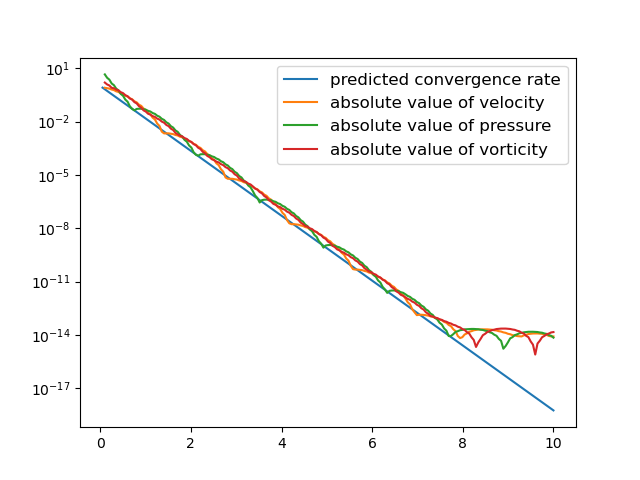
\includegraphics[width=\textwidth]{pic/rtp_cv.png}
    \caption{Return to zero flow}
    \label{fig:rtp_cv}
  \end{subfigure}
  \begin{subfigure}[b]{0.4\textwidth}
    \centering
    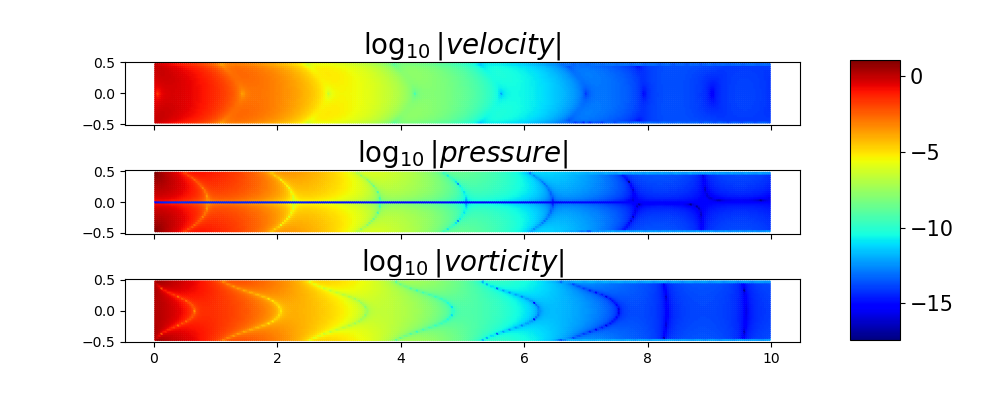
\includegraphics[width=\textwidth]{pic/rtppipe.png}
    \caption{Color plot of $\log_{10}$ of the absolute value of the velocity, vorticity, and pressure}
    \label{fig:rtppipe}
  \end{subfigure}
  \caption{Return to Poiseuille flow in a straight pipe. }
  \label{fig:r2pnumerical}
\end{figure}


\subsection{a complicated network of pipes to show the power of this method}



\section{Conclusions\label{sec:conclusions}}

\subsection{summarize what I've done}
\subsection{outlook. What other work might be followed?}
\bibliographystyle{plain}
\bibliography{references}


\end{document}
